\documentclass[border=5pt]{standalone}
\usepackage{pgfplots}
\pgfplotsset{compat=1.18}
\usepackage{siunitx}
\usepackage{tikz}
\usetikzlibrary{calc}

\definecolor{bs4}{RGB}{31,119,180}
\definecolor{bs8}{RGB}{255,127,14}
\definecolor{bs16}{RGB}{44,160,44}
\definecolor{bs32}{RGB}{214,39,40}

\begin{document}
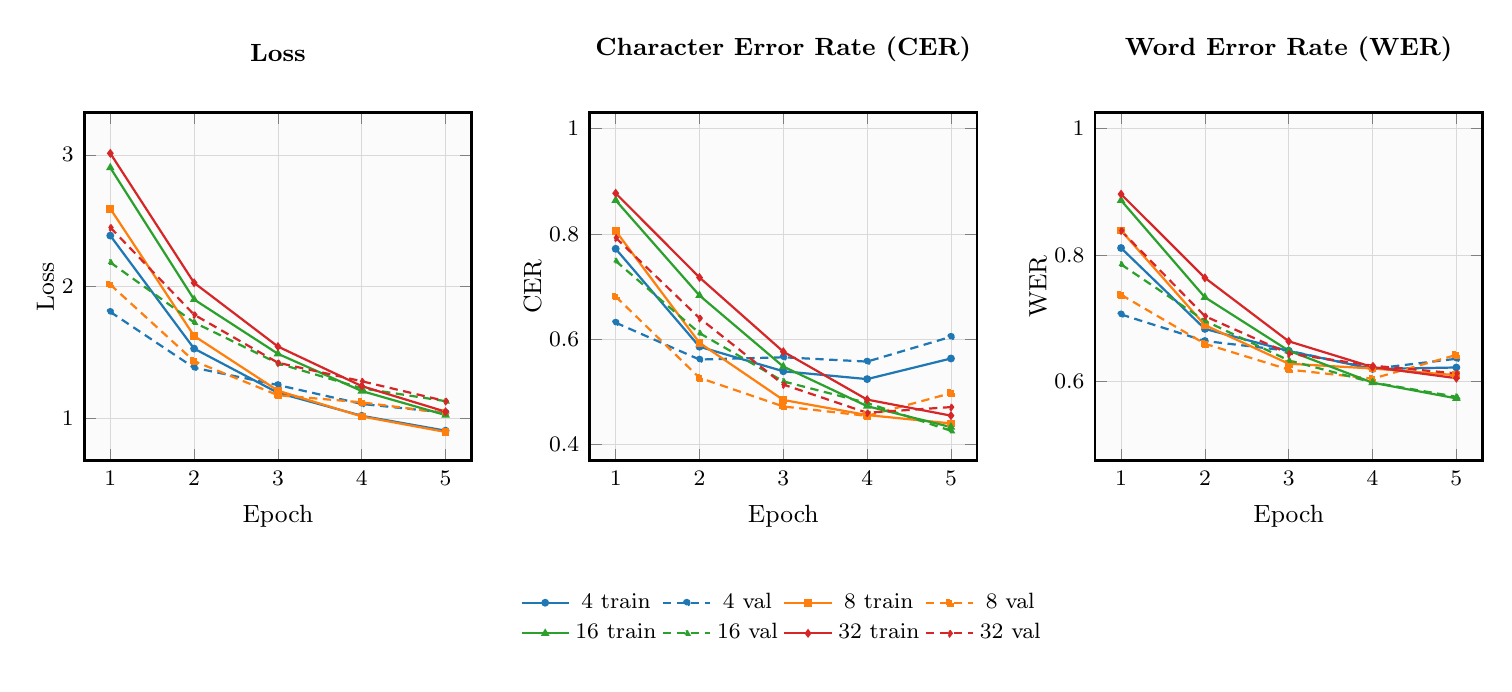
\begin{tikzpicture}[remember picture]

    % Графік 1: Loss
    \begin{axis}[
        name=plot1,
        width=6.5cm,
        height=6cm,
        xlabel={Epoch},
        ylabel={Loss},
        ylabel style={yshift=-0.15cm},
        xmin=0.9, xmax=5.1,
        ymin=0.8, ymax=3.2,
        xtick={1,2,3,4,5},
        grid=both,
        grid style={line width=.1pt, draw=gray!10},
        major grid style={line width=.2pt,draw=gray!30},
        title={Loss},
        axis background/.style={fill=gray!3},
        title style={yshift=3mm, font=\small\bfseries},
        label style={font=\small},
        tick label style={font=\footnotesize},
        line width=1pt,
        enlarge x limits=0.05,
        enlarge y limits=0.05,
        every axis plot/.append style={mark size=1pt}, % Reduced from 2pt to 1pt
        legend to name=commonlegend,
        legend columns=4,
        legend style={draw=none, fill=none, font=\footnotesize}
    ]
        % Batch size 4
        \addplot[color=bs4, mark=*, thick] coordinates {
            (1,2.3869) (2,1.5293) (3,1.1939) (4,1.0194) (5,0.9066)};
        \addplot[color=bs4, mark=*, thick, densely dashed] coordinates {
            (1,1.8081) (2,1.3842) (3,1.2529) (4,1.1096) (5,1.0436)};

        % Batch size 8
        \addplot[color=bs8, mark=square*, thick] coordinates {
            (1,2.5916) (2,1.6254) (3,1.2100) (4,1.0146) (5,0.8969)};
        \addplot[color=bs8, mark=square*, thick, densely dashed] coordinates {
            (1,2.0152) (2,1.4344) (3,1.1757) (4,1.1216) (5,1.0391)};

        % Batch size 16
        \addplot[color=bs16, mark=triangle*, thick] coordinates {
            (1,2.9021) (2,1.9021) (3,1.4900) (4,1.2074) (5,1.0251)};
        \addplot[color=bs16, mark=triangle*, thick, densely dashed] coordinates {
            (1,2.1837) (2,1.7281) (3,1.4173) (4,1.2285) (5,1.1307)};

        % Batch size 32
        \addplot[color=bs32, mark=diamond*, thick] coordinates {
            (1,3.0112) (2,2.0284) (3,1.5450) (4,1.2448) (5,1.0506)};
        \addplot[color=bs32, mark=diamond*, thick, densely dashed] coordinates {
            (1,2.4488) (2,1.7868) (3,1.4221) (4,1.2817) (5,1.1311)};

        \legend{4 train, 4 val, 8 train, 8 val, 16 train, 16 val, 32 train, 32 val}
    \end{axis}

    % Графік 2: CER, розташовується праворуч від plot1
    \begin{axis}[
        name=plot2,
        at={($(plot1.east)+(1.5cm,0)$)},
        anchor=west,
        width=6.5cm,
        height=6cm,
        xlabel={Epoch},
        ylabel={CER},
        ylabel style={yshift=-0.15cm},
        xmin=0.9, xmax=5.1,
        ymin=0.4, ymax=1.0,
        xtick={1,2,3,4,5},
        grid=both,
        grid style={line width=.1pt, draw=gray!10},
        major grid style={line width=.2pt,draw=gray!30},
        title={Character Error Rate (CER)},
        axis background/.style={fill=gray!3},
        title style={yshift=3mm, font=\small\bfseries},
        label style={font=\small},
        tick label style={font=\footnotesize},
        line width=1pt,
        enlarge x limits=0.05,
        enlarge y limits=0.05,
        every axis plot/.append style={mark size=1pt} % Reduced from 2pt to 1pt
    ]
        % Batch size 4
        \addplot[color=bs4, mark=*, thick] coordinates {
            (1,0.7717) (2,0.5859) (3,0.5394) (4,0.5245) (5,0.5636)};
        \addplot[color=bs4, mark=*, thick, densely dashed] coordinates {
            (1,0.6316) (2,0.5616) (3,0.5659) (4,0.5577) (5,0.6048)};

        % Batch size 8
        \addplot[color=bs8, mark=square*, thick] coordinates {
            (1,0.8056) (2,0.5933) (3,0.4849) (4,0.4563) (5,0.4404)};
        \addplot[color=bs8, mark=square*, thick, densely dashed] coordinates {
            (1,0.6812) (2,0.5269) (3,0.4726) (4,0.4547) (5,0.4978)};

        % Batch size 16
        \addplot[color=bs16, mark=triangle*, thick] coordinates {
            (1,0.8637) (2,0.6831) (3,0.5482) (4,0.4731) (5,0.4334)};
        \addplot[color=bs16, mark=triangle*, thick, densely dashed] coordinates {
            (1,0.7486) (2,0.6117) (3,0.5202) (4,0.4792) (5,0.4264)};

        % Batch size 32
        \addplot[color=bs32, mark=diamond*, thick] coordinates {
            (1,0.8771) (2,0.7173) (3,0.5765) (4,0.4856) (5,0.4552)};
        \addplot[color=bs32, mark=diamond*, thick, densely dashed] coordinates {
            (1,0.7928) (2,0.6402) (3,0.5142) (4,0.4606) (5,0.4714)};
    \end{axis}

    % Графік 3: WER, розташовується праворуч від plot2
    \begin{axis}[
        name=plot3,
        at={($(plot2.east)+(1.5cm,0)$)},
        anchor=west,
        width=6.5cm,
        height=6cm,
        xlabel={Epoch},
        ylabel={WER},
        ylabel style={yshift=-0.15cm},
        xmin=0.9, xmax=5.1,
        ymin=0.5, ymax=1.0,
        xtick={1,2,3,4,5},
        grid=both,
        grid style={line width=.1pt, draw=gray!10},
        major grid style={line width=.2pt,draw=gray!30},
        title={Word Error Rate (WER)},
        axis background/.style={fill=gray!3},
        title style={yshift=3mm, font=\small\bfseries},
        label style={font=\small},
        tick label style={font=\footnotesize},
        line width=1pt,
        enlarge x limits=0.05,
        enlarge y limits=0.05,
        every axis plot/.append style={mark size=1pt} % Reduced from 2pt to 1pt
    ]
        % Batch size 4
        \addplot[color=bs4, mark=*, thick] coordinates {
            (1,0.8110) (2,0.6831) (3,0.6482) (4,0.6198) (5,0.6221)};
        \addplot[color=bs4, mark=*, thick, densely dashed] coordinates {
            (1,0.7060) (2,0.6640) (3,0.6485) (4,0.6200) (5,0.6359)};

        % Batch size 8
        \addplot[color=bs8, mark=square*, thick] coordinates {
            (1,0.8386) (2,0.6890) (3,0.6281) (4,0.6205) (5,0.6099)};
        \addplot[color=bs8, mark=square*, thick, densely dashed] coordinates {
            (1,0.7371) (2,0.6596) (3,0.6188) (4,0.6044) (5,0.6420)};

        % Batch size 16
        \addplot[color=bs16, mark=triangle*, thick] coordinates {
            (1,0.8863) (2,0.7331) (3,0.6487) (4,0.5981) (5,0.5733)};
        \addplot[color=bs16, mark=triangle*, thick, densely dashed] coordinates {
            (1,0.7851) (2,0.6959) (3,0.6334) (4,0.5985) (5,0.5758)};

        % Batch size 32
        \addplot[color=bs32, mark=diamond*, thick] coordinates {
            (1,0.8961) (2,0.7638) (3,0.6635) (4,0.6228) (5,0.6052)};
        \addplot[color=bs32, mark=diamond*, thick, densely dashed] coordinates {
            (1,0.8385) (2,0.7033) (3,0.6442) (4,0.6250) (5,0.6128)};
    \end{axis}

    % Розміщення загальної легенди під усіма графіками
    \node at ($(plot1.south)!0.5!(plot3.south)+(0,-2.0cm)$) {\pgfplotslegendfromname{commonlegend}};
    
\end{tikzpicture}
\end{document}